\chapter{Work Plan}
\label{chap:WorkPlan}

The execution of this dissertation followed a structured 12-month plan, commencing in November 2024 and culminating in the submission in October 2025. This chapter outlines the strategic phasing of the project, designed to ensure a logical progression from foundational research to final implementation and evaluation.

The timeline was organized into five distinct but overlapping phases, each with specific objectives and deliverables. This approach facilitated agile adaptation while maintaining a clear focus on the project's long-term goals. The complete project schedule, including granular tasks and their dependencies, is visualized in the Gantt chart presented in Figure~\ref{fig:gantt_chart_detailed}.

\begin{figure}[htbp]
    \centering
    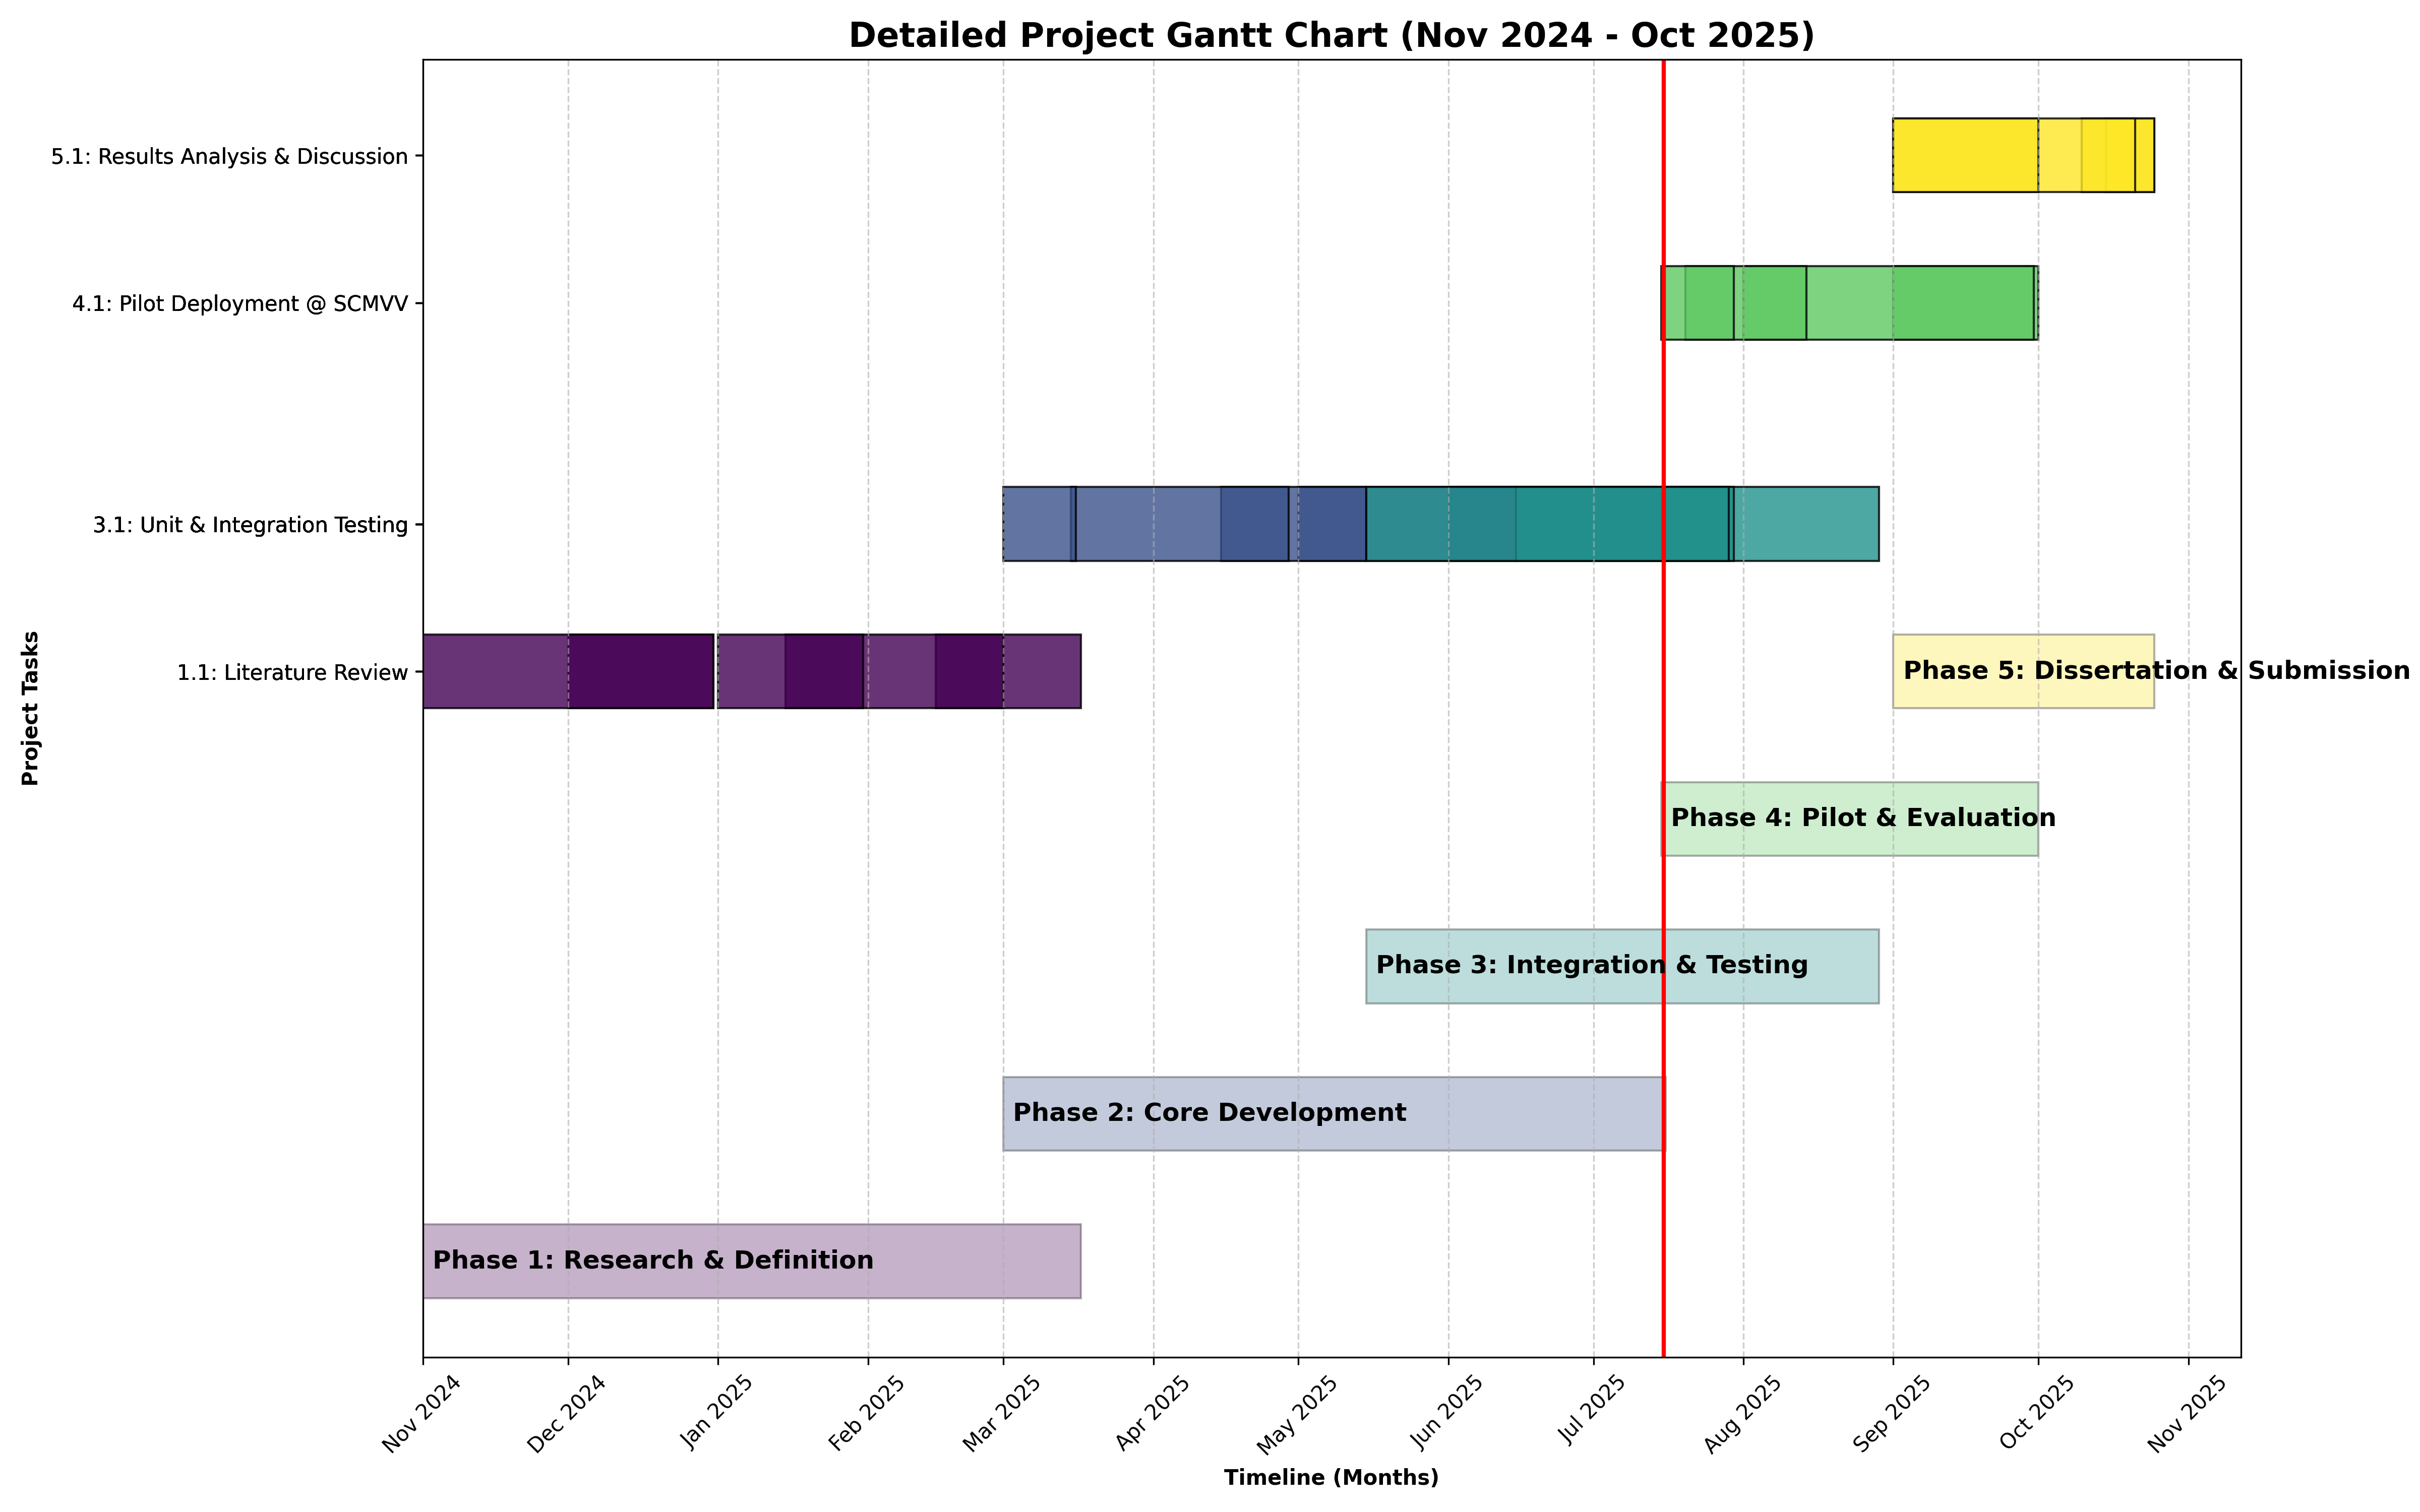
\includegraphics[width=\textwidth]{images/generated/gantt_chart_detailed.png}
    \caption{Detailed Gantt chart illustrating the 12-month project timeline, key phases, and task dependencies from November 2024 to October 2025.}
    \label{fig:gantt_chart_detailed}
\end{figure}

The initial phase, \textbf{Research and Definition}, focused on establishing a solid theoretical and empirical foundation through an exhaustive literature review and an in-depth analysis of the existing clinical workflows at SCMVV. This was followed by the \textbf{Core Development} phase, where the system's foundational components, including the database, security modules, and core backend logic, were implemented.

Subsequently, the \textbf{Integration and Testing} phase ensured that the newly developed modules operated cohesively and could be reliably connected to existing external and legacy systems. The fourth phase, \textbf{Pilot and Evaluation}, marked the transition from a development environment to a live clinical setting, where the system was deployed and rigorously evaluated based on user feedback and performance data.

The final phase, \textbf{Dissertation and Submission}, was dedicated to the analysis of the collected data, the synthesis of the research findings, and the writing of this dissertation, culminating in its final submission and defense. The detailed methodological framework underpinning the execution of this plan is elaborated upon in the following chapter. 